% Created 2015-03-15 Sun 13:38
\documentclass{article}
\usepackage[utf8]{inputenc}
\usepackage[T1]{fontenc}
\usepackage{fixltx2e}
\usepackage{graphicx}
\usepackage{longtable}
\usepackage{float}
\usepackage{wrapfig}
\usepackage{rotating}
\usepackage[normalem]{ulem}
\usepackage{amsmath}
\usepackage{textcomp}
\usepackage{marvosym}
\usepackage{wasysym}
\usepackage{amssymb}
\usepackage{capt-of}
\usepackage{hyperref}
\tolerance=1000
\author{Christopher Findeisen \& Sam Gwydir \& Jerego Orlino \& Vincent Valenti}
\date{\today}
\title{Eugenics-System Design Document}
\hypersetup{
 pdfkeywords={},
  pdfsubject={},
  pdfcreator={Emacs 24.4.90.1 (Org mode 8.3beta)}}
\begin{document}

\maketitle
\begin{abstract}
In this document we present our design for an AI that is capable of generating
circuits and visualizing the process.
\end{abstract}

\setcounter{tocdepth}{2}
\tableofcontents
\pagebreak

\section{Purpose}
\label{sec-1}

Project 3 explores Artificial Intelligence, or AI. The AI detailed herein
generates a circuit equivalent to a given logic function using one of two
algorithms. We have dubbed our AI system "eugenics".


The eugenics system implements two search algorithms to solve this problem, the
first is genetic, and the second (hereafter referred to as traditional) takes
advantage of Karnaugh Maps to generate an optimal representation of the given
logic function, then uses a search algorithm to find a circuit that fits the
constraints given. We have named our genetics algorithm "HMS Beagle" and the
traditional algorithm "Karnaughvor". Finding the humor the former is an
exercises left to the reader.

An additional point of interest is comparing the performance
of these two approaches.

This system could be useful in minimizing circuits for electrical engineers,
though it is of limited use because it does not make any effort to recognize any
sort of hazard. The program could be used as a library if one wanted to create a
circuit synthesizer for use in implementing an arbitrary logic function on an
FPGA. However the scope of this project limits its use in physical
applications.

The visualization provided would be educational to those studying genetic
algorithms.

\section{Definitions}
\label{sec-2}

\begin{description}
\item[{Circuit}] A circuit is a collection of gates, inputs and outputs.

\item[{Sub-Circuit}] A sub-circuit is a proper subset of a circuit.

\item[{Circuit Candidate}] A circuit candidate is the output of a step of the algorithm performed by the
engine. It is a circuit that is being tested if it is equivalent to our desired
outcome.
\end{description}

\section{Constraints}
\label{sec-3}
There are three constraints that have been explicitly stated:

\begin{enumerate}
\item Each circuit may only contain AND, OR, and NOT gates.
\item There can be any number of AND and OR gates, but no more than two NOT gates.
\item AND and OR can have any number of inputs.
\end{enumerate}

\section{High Level Entities}
\label{sec-4}

\subsection{Algorithm}
\label{sec-4-1}

\subsubsection{Genetic Algorithm}
\label{sec-4-1-1}
The genetic algorithm will generate a large population of candidate circuits,
splice them together randomly, and if they are "fit", they will move on into the
next generation of candidates. This process continues until we reach the desired
circuit.

\subsubsection{Traditional Algorithm}
\label{sec-4-1-2}
The traditional algorithm will start by generating a Karnaugh Map which will
serve as the algorithms' starting point. A Karnaugh Map provides the optimal
representation of a circuit when one groups the outputs using the rules it
defines. These rules ask the user to group adjacent 1's together in groups of
2\(^{\text{n}}\). We will use a search algorithm to find a set of rules/groups that cause the
map to generate a function (and therefore circuit) that fits our constraints.

\subsection{Server-Client Model}
\label{sec-4-2}

\begin{figure}[hp]
\centering
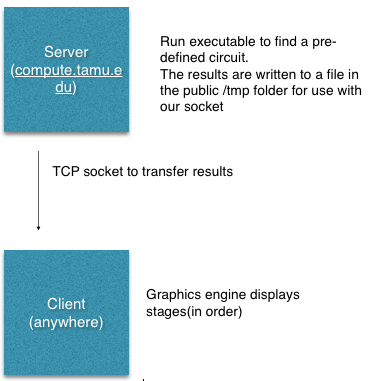
\includegraphics[width={.50\textwidth}]{../img/clientserver.png}
\caption{\label{fig:servclie}Eugenics-System Model Diagram}
\end{figure}

\subsubsection{Circuit Engine Server}
\label{sec-4-2-1}
The Circuit Engine server is the work horse of the Eugenics system. It performs
the algorithm specified and writes the current candidate (the current circuit)
in real-time to a TCP-socket which the Visualization client listens on.

\subsubsection{Visualization Client}
\label{sec-4-2-2}
The Visualization client uses the FLTK graphics library to display a graphical
representation of the current sub-circuit. This will be used to analyze the
progress of the genetic algorithm in near real-time.

The client listens to the Circuit engine server over a TCP-socket and generates
a graphical representation using the client computer's graphics card.

\section{Low Level Design}
\label{sec-5}

\subsection{Logic Gate}
\label{sec-5-1}
A gate is an object that has a set of inputs and outputs and assigns the outputs
according to its operation. The logic gate is the simplest form of sub-circuit.
There are three types of gates, the n-ary, unary, and binary gates.

The n-ary gate has n inputs and one output. It performs its operation on its
inputs and produces its output. The operation can either be logical AND or
logical OR. Because a n-ary gate can be formed by daisy-chaining binary gates,
we will always break it down into its constituent binary gates. This leaves us
with two types of gates. \\

The two types of gates are:
\begin{description}
\item[{the binary gate}] A binary gate has two inputs and one output where output = op(input). Op is
either logical AND or logical OR.
\item[{the unary gate}] A unary gate has one input and one output where output = op (input). Because
there is only one unary gate, op is always logical NOT.
\end{description}

\subsection{Sub-Circuit}
\label{sec-5-2}

\begin{figure}[hp]
\centering
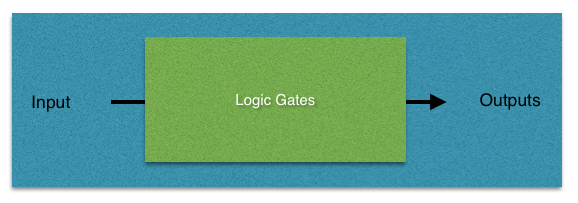
\includegraphics[width={.50\textwidth}]{../img/circuit.png}
\caption{\label{fig:circ}Sub-Circuit Abstraction Diagram}
\end{figure}

A sub-circuit is a proper subset of a circuit.

A sub-circuit is an object that contains a set of sub-circuits and their input
and output connections. The sub-circuit itself has a set of inputs and outputs
which are supersets of the contained gates inputs and outputs, respectively.

A sub-circuit has a function to evaluate it self which maps its inputs to the
outputs by applying its gates as operations on the inputs. \\

There are three base cases for a sub-circuit:
\begin{description}
\item[{a gate}] A gate either a binary or unary gate.
\item[{an input/output terminal}] An input or output terminal is a node at either extreme of the circuit. The
input nodes can be arbitrarily assigned a set of input values where each input
can be 0 or 1. The set of outputs will take on values as a function of the
inputs. These are not to be confused with intermediate outputs and inputs, which
are values on a wire between two gates.
\item[{a logical value (only used during evaluation)}] When a sub-circuit is evaluated during circuit evaluation, it becomes its
output value. This is useful when recursively evaluating circuits.
\end{description}

\subsection{Circuit}
\label{sec-5-3}

A circuit is a proper superset of all sub-circuits in a candidate.

Note that a circuit is itself a sub-circuit where the inputs set and output set
are equal in magnitude to the given logic function. However to avoid confusion
we will never refer to a circuit as a sub-circuit.

A circuit can evaluate itself by recursively evaluating its set of
sub-circuits.

The underlying data structure for a circuit will be a tree in which the root is
a sub-circuit where its set of outputs are set containing the output terminals,
note that there can be more outputs than in the desired circuit, but never less.

A parent node in the tree can have any number of children sub-circuits.  The
children are the sub-circuits where their set of outputs contain the inputs of
their parent.

The leaves of the tree will always be the input terminals.

When a circuit is evaluated with a set of input values, it becomes the set of
its outputs. This is useful when evaluating whether or not the circuit is
equivalent to the desired circuit.

\subsection{Visualization}
\label{sec-5-4}

The graphic engine will display the current state of the system periodically.
We'll update once every n mutations with the Genetic algorithm, and once every
change within the Traditional algorithm.

The number of iterations between each display of the current circuit n, will be
determined experimentally and will be as low as possible to keep the
visualization as near real-time as possible.

\section{Configuration}
\label{sec-6}

\begin{itemize}
\item The desired logic function must be well-defined. Our design does not account for
"don't cares" in the desired circuits truth-table.

\item Depending on the compute server's configuration, some additional configuring may
be necessary in order to compile and link libraries correctly.

\item Additionally, the compute server will need to be live in order for the
client to connect to the server.
\end{itemize}

\section{Benefits, Assumptions, and Risks}
\label{sec-7}

\subsection{Benefits}
\label{sec-7-1}

\begin{itemize}
\item The client-server separation allows us to view the running program from any
machine. This also provides us with access to more powerful graphics cards,
allowing us to set n lower and display closer to real-time.

\item The circuit model abstracts the data into a tree structure which is easily
traverseable.
\end{itemize}

\subsection{Assumptions}
\label{sec-7-2}

\begin{itemize}
\item The problems will always be pre-defined. (no "don't cares")

\item The compute.tame.edu server is up.

\item Compute allows us the permissions to set up a server on the internet.
\end{itemize}

\subsection{Risks}
\label{sec-7-3}

\begin{itemize}
\item Compute or CS department rules do not let us set up a server on compute.

\item Can lead to large network i/o, which could lead to shutdown by compute sysadmins.

\item We're using many libraries, so there is always a risk incurred that those
builds/configs will be difficult to test and/or not work on the TA's account
due to a wrong assumption about the TA's shell environment.
\end{itemize}

\section{References}
\label{sec-8}
\begin{description}
\item[{How to write an effective design document}] 
\end{description}
\url{http://blog.slickedit.com/2007/05/how-to-write-an-effective-design-document/}
% Emacs 24.4.90.1 (Org mode 8.3beta)
\end{document}